\section{Verschillen Tussen Talen}

\subsection{Turing Completeness}

\begin{frame}
  \tableofcontents[currentsection]
\end{frame}

\begin{frame}
  \frametitle{Turing Completeness}
  \begin{itemize}
    \item Hoe ``krachtig'' is een taal?
    \item Zijn er talen die meer kunnen dan andere?
    \item Kan een programma geschreven in taal X ook geschreven worden in taal Y?
  \end{itemize}
\end{frame}

\begin{frame}
  \frametitle{Turing Completeness}
  \begin{itemize}
    \item Een taal is Turing complete indien elk mogelijk programma erin kan geschreven worden
    \item (Zo goed als) Alle talen zijn Turing complete
    \item M.a.w.~(bijna) alle talen zijn equivalent qua ``kracht''
  \end{itemize}
\end{frame}

\begin{frame}
  \frametitle{Visualisatie}
  \begin{center}
    \begin{tikzpicture}
      \shade [left color=red,right color=green] (0,0) rectangle (10,0.2);
      \node[anchor=north east,rotate=90] at (0,0) {\parbox{2cm}{\flushright Turing \\ incomplete}};
      \node[anchor=south east,rotate=90] at (10,0) {\parbox{2cm}{\flushright Turing \\ complete}};

      \node[language] at (9,1) {\cpp};
      \node[language] at (9,2) {Java};
      \node[language] at (9,3) {\csharp};
      \node[language] at (9,4) {Python};
      \node[language] at (9,5) {\dots};
      \node[language] at (1,1) {Coq};
    \end{tikzpicture}
  \end{center}
\end{frame}


\subsection{Effici\"entie}

\begin{frame}
  \tableofcontents[currentsubsection]
\end{frame}

\begin{frame}
  \frametitle{Effici\"entie}
  \begin{itemize}
    \item Sommige talen focussen zuiver op snelheid van uitvoering
    \item Geen poging om veilig te zijn
    \item C/\cpp\ zien snelheid als topprioriteit
  \end{itemize}
  \begin{center}
    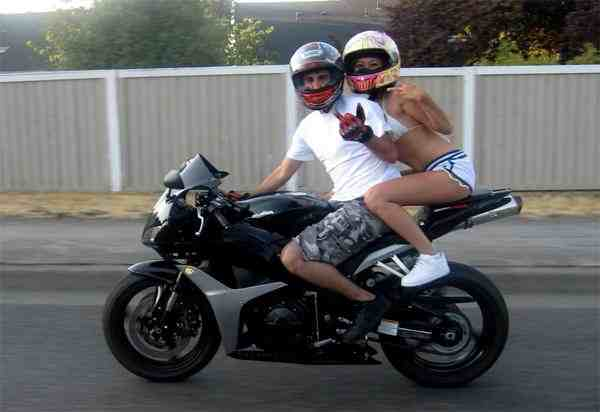
\includegraphics[width=5cm]{unsafe-driving.jpg}
  \end{center}
\end{frame}

\begin{frame}
  \frametitle{Effici\"entie}
  \begin{itemize}
    \item Veel talen offeren snelheid op voor veiligheid
    \item Checken constant op mogelijke fouten tijdens uitvoering
    \item Bv.~\csharp, Java
  \end{itemize}
  \begin{center}
    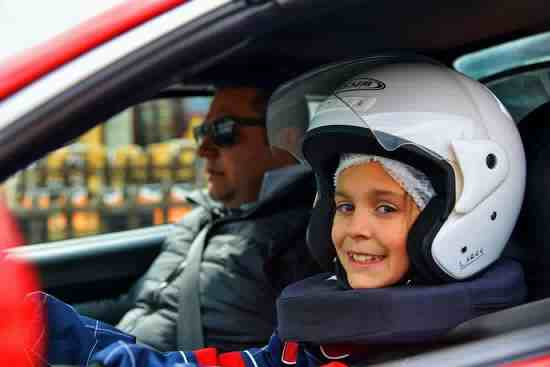
\includegraphics[width=5cm]{drive-safely.jpg}
  \end{center}
\end{frame}

\begin{frame}
  \frametitle{Effici\"entie}
  \begin{itemize}
    \item Andere talen verkiezen comfort en flexibiliteit
    \item Kunnen 100$\times$ trager zijn dan C/C++
    \item Bv.~Ruby, Python, Common Lisp
  \end{itemize}
  \begin{center}
    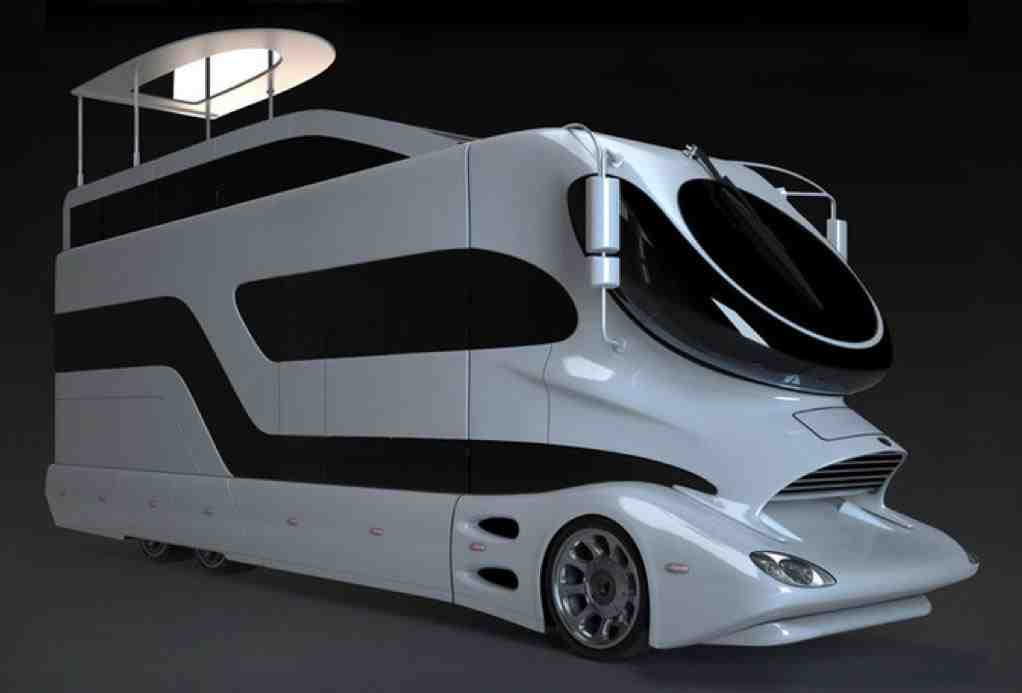
\includegraphics[width=5cm]{luxury-driving.jpg}
  \end{center}
\end{frame}

\begin{frame}
  \frametitle{Visualisatie}
  \begin{center}
    \begin{tikzpicture}
      \shade [left color=red,right color=green] (0,0) rectangle (10,0.2);
      \node[anchor=north east,rotate=90] at (0,0) {Traag};
      \node[anchor=south east,rotate=90] at (10,0) {Snel};

      \node[language] at (9,1) {C};
      \node[language] at (9,2) {\cpp};
      \node[language] at (8,3) {Rust};
      \node[language] at (8,4) {O'Caml};
      \node[language] at (6,1) {Java};
      \node[language] at (7,2) {\csharp};
      \node[language] at (3,1) {Python};
      \node[language] at (4,3) {Javascript};
      \node[language] at (5,4) {Haskell};
      \node[language] at (2,2) {Ruby};
    \end{tikzpicture}
  \end{center}
\end{frame}

\subsection{Bugdetectie}

\begin{frame}
  \tableofcontents[currentsubsection]
\end{frame}

\begin{frame}
  \frametitle{Bugdetectie}
  \begin{itemize}
    \item Schrijven van code is niet eenvoudig
    \item Bugs onvermijdelijk
    \item Hoe kunnen we met bugs omgaan?
  \end{itemize}
\end{frame}

\begin{frame}
  \frametitle{Optie \#1: Bugs Volledig Vermijden}
  \begin{itemize}
    \item Wiskundige analyses loslaten op code
    \item Programma pas uitgeven als 100\%\ correctheid bewezen is
    \item Heet ``compile time checking''
  \end{itemize}
  \vskip4mm
  \structure{Voor- en Nadelen}
  \begin{itemize}
    \item[\pro] Klant krijgt perfect werkend product
    \item[\con] Kost gigantisch veel moeite
          \begin{itemize}
            \item Bv.~taal Coq
            \item Productiviteit 100$\times$ lager
          \end{itemize}
  \end{itemize}
  \vskip4mm
  \structure{In de Praktijk}
  \begin{itemize}
    \item Belangrijk voor ziekenhuissoftware, vliegtuigen, \dots
  \end{itemize}
\end{frame}

\begin{frame}
  \frametitle{Optie \#2: Bugs Detecteren Tijdens Uitvoering}
  \begin{itemize}
    \item Tijdens uitvoering situatie constant monitoren
    \item Indien iets niet klopt: situatie herstellen of alles stopzetten
    \item Heet ``runtime checking''
  \end{itemize}
  \vskip4mm
  \structure{Voor- en Nadelen}
  \begin{itemize}
    \item[\pro] Goedkoper om te ontwikkelen
    \item[\con] Klant krijgt buggy programma
    \item[\con] Programma werkt trager, vergt meer geheugen
  \end{itemize}
\end{frame}

\begin{frame}
  \frametitle{Optie \#3: Bugs Negeren}
  \begin{itemize}
    \item Ervan uitgaan dat er gewoon geen bugs zijn
    \item Indien wel bug: blijven doorgaan
  \end{itemize}
  \vskip4mm
  \structure{Voor- en Nadelen}
  \begin{itemize}
    \item[\pro] Goedkoop om te ontwikkelen
    \item[\pro] Programma draait heel effici\"ent
    \item[\con] Klant krijgt foute resultaten zonder het te beseffen
  \end{itemize}
\end{frame}

\begin{frame}
  \frametitle{Visualisatie}
  \begin{center}
    \begin{tikzpicture}[scale=.75,transform shape,
                        header/.style={fill=gray,minimum width=2cm,minimum height=0.75cm,font=\scshape}]
      \shade [left color=red,right color=green] (-0.2,0) rectangle (10,-0.2);
      \shade [left color=red,right color=green,shading angle=180] (0,-0.2) rectangle (-0.2,5);
      \draw[thick] (0,5) -- (10,0);
      
      \node[header,anchor=north west] at (-0.2,-0.2) {Compile-Time};
      \node[header,anchor=south west,rotate=90] at (-0.2,-0.2) {Runtime};

      \node[language] at (5,0) {C/\cpp};
      \node[language] at (7.5,1.25) {Rust};
      \node[language] at (10,0) {Coq};
      \node[language] at (5,3.75) {Java};
      \node[language] at (5,2.5) {\csharp};
      \node[language] at (2.5,3) {TypeScript};
      \node[language] at (0,3) {Javascript};
      \node[language] at (0,5) {Python, Ruby};
      \node[language] at (0,0) {Machinetaal};
    \end{tikzpicture}
  \end{center}

  \begin{overprint}
    \onslide<1>
    \begin{center}
      De meeste talen combineren compile-time met runtime checks \\ (bv. \csharp, Java, TypeScript, Rust)
    \end{center}

    \onslide<2>
    \begin{center}
      Python, Ruby en Javascript voeren enkel checks uit at runtime
    \end{center}

    \onslide<3>
    \begin{center}
      Coq voert alle checks uit at compile-time
    \end{center}

    \onslide<4>
    \begin{center}
      C, \cpp\ voeren compile-time checks uit, maar slechts gedeeltelijk. Heel wat bugs blijven ongedecteerd
    \end{center}

    \onslide<5>
    \begin{center}
      Machinetaal scoort erbarmelijk
    \end{center}
  \end{overprint}
\end{frame}

\subsection{Libraries}

\begin{frame}
  \tableofcontents[currentsubsection]
\end{frame}

\begin{frame}
  \frametitle{Libraries}
  \begin{itemize}
    \item Taal laat toe om woordenschat uit te breiden
    \item Technische term: libraries
          \begin{itemize}
            \item Beeld en geluid
            \item GUIs
            \item Webapplicaties
            \item \dots
          \end{itemize}
    \item Men kan zelf libraries beginnen schrijven
    \item Of men kan voortwerken op het werk van anderen
    \item Verschillende talen hebben verschillende reeds bestaande libraries
  \end{itemize}
\end{frame}

\begin{frame}
  \frametitle{Libraries}
  \structure{Ruby}
  \begin{itemize}
    \item Ruby is vooral gekend voor \'e\'en specifieke library
          \begin{itemize}
            \item Ruby on Rails voor ontwikkeling webapplicaties
          \end{itemize}
    \item Maar Ruby heeft bv.~niet echt een deftige GUI library
  \end{itemize}
  \vskip4mm
  \structure{Javascript}
  \begin{itemize}
    \item In theorie ken elke taal in een browser werken
    \item In de praktijk: slechts beperkt aantal talen
          \begin{itemize}
            \item Javascript
            \item TypeScript
            \item Dart
          \end{itemize}
  \end{itemize}
\end{frame}

\begin{frame}
  \frametitle{Libraries}
  \structure{Python}
  \begin{itemize}
    \item Python staat gekend om zijn veelheid aan libraries
    \item Populair om snel dingen gedaan te krijgen
    \item Zwitsers zakmes onder de programmeertalen
  \end{itemize}
  \vskip4mm
  \structure{Erlang}
  \begin{itemize}
    \item Gespecialiseerd in gedistribueerde systemen
          \begin{itemize}
            \item Software die op meerdere met elkaar communicerende machines draait
          \end{itemize}
  \end{itemize}
\end{frame}

\subsection{Andere Aspecten}

\begin{frame}
  \tableofcontents[currentsubsection]
\end{frame}

\begin{frame}
  \frametitle{Gebruiksgemak}
  \begin{itemize}
    \item Hoe gemakkelijk/moeilijk is de taal?
    \item Hoe goed is de documentatie?
    \item Wat voor tools zijn er beschikbaar?
          \begin{itemize}
            \item Editors
            \item Debuggers
            \item Package managers
            \item Linters
            \item \dots
          \end{itemize}
  \end{itemize}
  \begin{center}
    \begin{tikzpicture}[scale=.75,transform shape,
                        header/.style={fill=gray,minimum width=2cm,minimum height=0.75cm,font=\scshape}]
      \shade [left color=red,right color=green] (0,-0.4) rectangle (10,-0.2);
      
      \node[header,anchor=north west] at (0,-0.4) {Moeilijk};
      \node[header,anchor=north east] at (10,-0.4) {Gemakkelijk};

      \node[language,rotate=90,anchor=north west] at (0,0) {Machinetaal, Coq};
      \node[language,rotate=90,anchor=north west] at (3,0) {C};
      \node[language,rotate=90,anchor=north west] at (2,0) {\cpp};
      \node[language,rotate=90,anchor=north west] at (5,0) {Java};
      \node[language,rotate=90,anchor=north west] at (6,0) {\csharp};
      \node[language,rotate=90,anchor=north west] at (7,0) {TypeScript};
      \node[language,rotate=90,anchor=north west] at (8,0) {Javascript};
      \node[language,rotate=90,anchor=south west] at (10,0) {Python, Ruby};
    \end{tikzpicture}
  \end{center}
\end{frame}

\begin{frame}
  \frametitle{Teamwork}
  \begin{itemize}
    \item Sommige talen zijn enkel geschikt voor kleine teams
    \item Andere bieden ondersteuning voor grote teams
  \end{itemize}

  \begin{center}
    \begin{tikzpicture}[scale=.75,transform shape,
                        header/.style={fill=gray,minimum width=2cm,minimum height=0.75cm,font=\scshape}]
      \shade [left color=red,right color=green] (0,-0.4) rectangle (10,-0.2);
      
      \node[header,anchor=north west] at (0,-0.4) {Kleine teams};
      \node[header,anchor=north east] at (10,-0.4) {Grote teams};

      \node[language,rotate=90,anchor=north west] at (0,0) {Machinetaal};
      \node[language,rotate=90,anchor=north west] at (3,0) {C};
      \node[language,rotate=90,anchor=north west] at (8,0) {\cpp};
      \node[language,rotate=90,anchor=north west] at (7,0) {\csharp};
      \node[language,rotate=90,anchor=north west] at (6,0) {Java};
      \node[language,rotate=90,anchor=north west] at (2,0) {Python, Ruby};
      \node[language,rotate=90,anchor=north west] at (1,0) {Javascript};
      \node[language,rotate=90,anchor=south west] at (5,0) {Haskell};
    \end{tikzpicture}
  \end{center}
\end{frame}

\begin{frame}
  \frametitle{Low vs High Level}
  \begin{itemize}
    \item Sommige talen verbergen details van de machine
    \item Andere geven toegang tot de ``organen'' van de machine
  \end{itemize}

  \begin{center}
    \begin{tikzpicture}[scale=.75,transform shape,
                        header/.style={fill=gray,minimum width=2cm,minimum height=0.75cm,font=\scshape}]
      \shade [left color=red,right color=green] (0,-0.4) rectangle (10,-0.2);
      
      \node[header,anchor=north west] at (0,-0.4) {Low level};
      \node[header,anchor=north east] at (10,-0.4) {High level};

      \node[language,anchor=south] at (0,0) {Machinetaal};
      \node[language,anchor=south west] at (0,1) {C};
      \node[language,anchor=south west,minimum width=10cm] at (0,2) {\cpp};
      \node[language,anchor=south west,minimum width=5cm] at (3,1) {\csharp};
      \node[language,anchor=south west] at (4,0) {Java};
      \node[language,anchor=south west] at (7,0) {Python};
      \node[language,anchor=south west] at (7,3) {Javascript};
      \node[language,anchor=south west,minimum width=5cm] at (1,3) {Rust};
      \node[language,anchor=south west] at (7,4) {TypeScript};
      \node[language,anchor=south west,minimum width=2cm] at (2,4) {Go};
    \end{tikzpicture}
  \end{center}
\end{frame}


%%% Local Variables:
%%% mode: latex
%%% TeX-master: "programming-languages"
%%% End:
